\documentclass[crop=false, class=book]{standalone}

%pacchetto per immagini
\usepackage{graphicx}
\usepackage{subfig}

\usepackage[italian]{varioref}
\usepackage{copyrightbox}
\usepackage{url}

\usepackage{enumitem}
\newcommand\litem[1]{\item{\bfseries #1:}}


\begin{document}
	\chapter{Cloud anchors}
	L'API ARCore \textit{Cloud Anchor} introduce i cloud anchor, un tipo speciale di anchor che permettono di condividere con altri utenti l'esperienza AR. In particolare, un dispositivo può posizionare oggetti virtuali nello spazio, e altri utenti possono vedere l'oggetto virtuale ed interagire con esso trovandosi nella stessa posizione, come spiegato da \cite{kert2021mobile}.
	\\
	Questo tipo di anchor, come spiegato dalla documentazione ufficiale \cite{google2022cloud}, trova applicazione ad esempio per creare oggetti virtuali che persistano nel mondo reale, cioè che mantengano nel tempo la posizione in cui sono stati creati, oppure per creare giochi virtuali multigiocatore in cui è importante la collaborazione tra utenti in tempo reale.
	
	\section{Funzionamento}
	La creazione e la diffusione dell'anchor avviene tramite connessione internet in quattro passaggi, descritti ad alto livello come segue. La figura~\vref{fig:cloud} tratta dalla guida ufficiale Google descrive visivamente le quattro fasi del funzionamento dei cloud anchor.
	\begin{enumerate}
		\litem{Creation} l'utente crea un anchor localmente;
		\litem{Hosting} ARCore carica i dati della mappa 3D dello spazio circostante all'anchor locale nell'ARCore Cloud Anchor, che a sua volta restituisce al dispositivo un Cloud Anchor ID univoco;
		\litem{Distribution} l'app distribuisce l'ID univoco agli altri utenti;
		\litem{Resolving} gli utenti possono utilizzare l'ID ricevuto per ricreare l'anchor quando si trovano nello stesso ambiente. L'API compara la scena del dispositivo con la mappa 3D caricata precedentemente per determinare la posizione dell'utente e visualizzare correttamente l'oggetto virtuale.
	\end{enumerate}
	
	\begin{figure}
		\centering
		\subfloat[][\emph{Creazione dell'anchor locale.}]
		{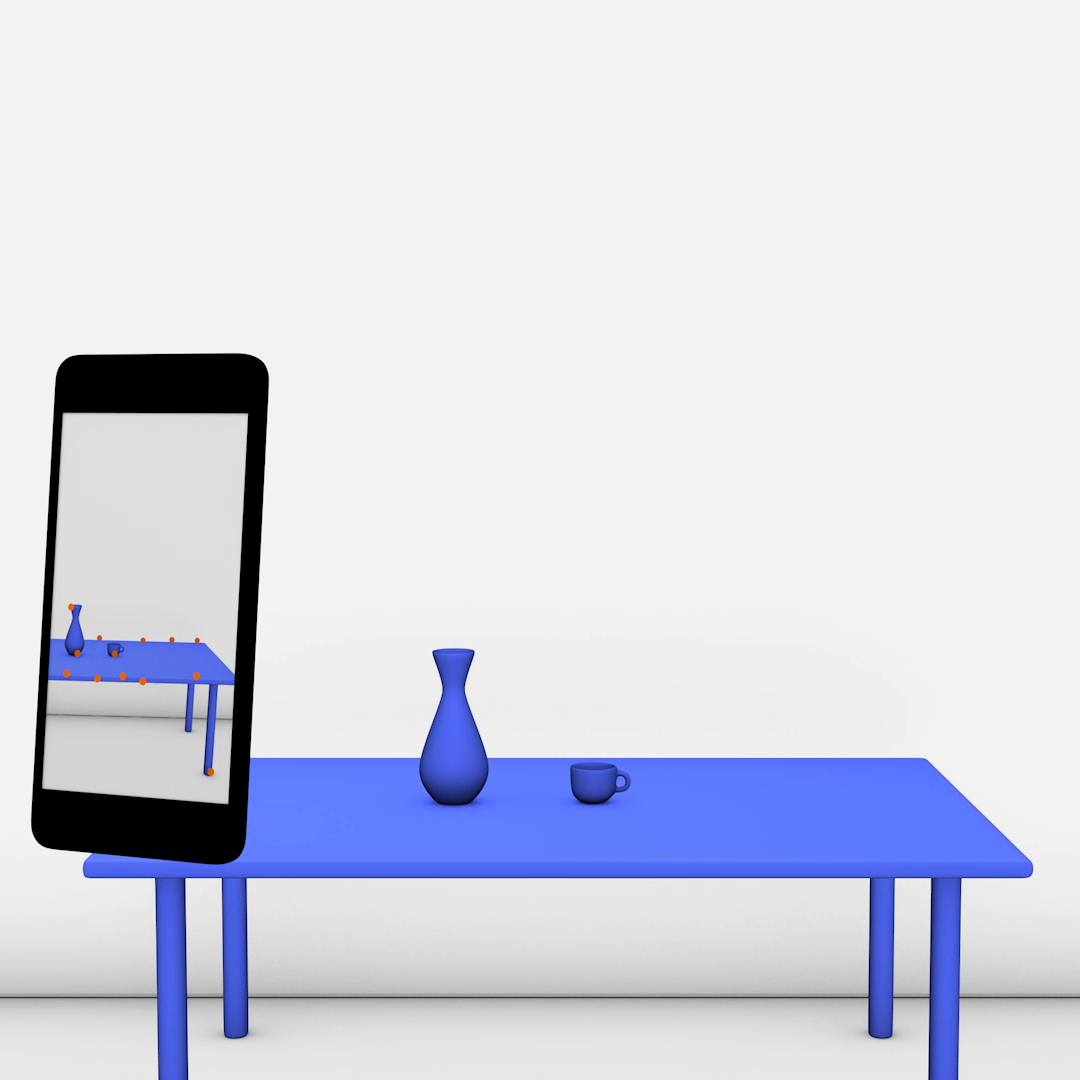
\includegraphics[width=0.45\textwidth]{./resources/images/cloud_anchors/creation}}  \quad
		\subfloat[][\emph{Hosting dell'anchor.}]
		{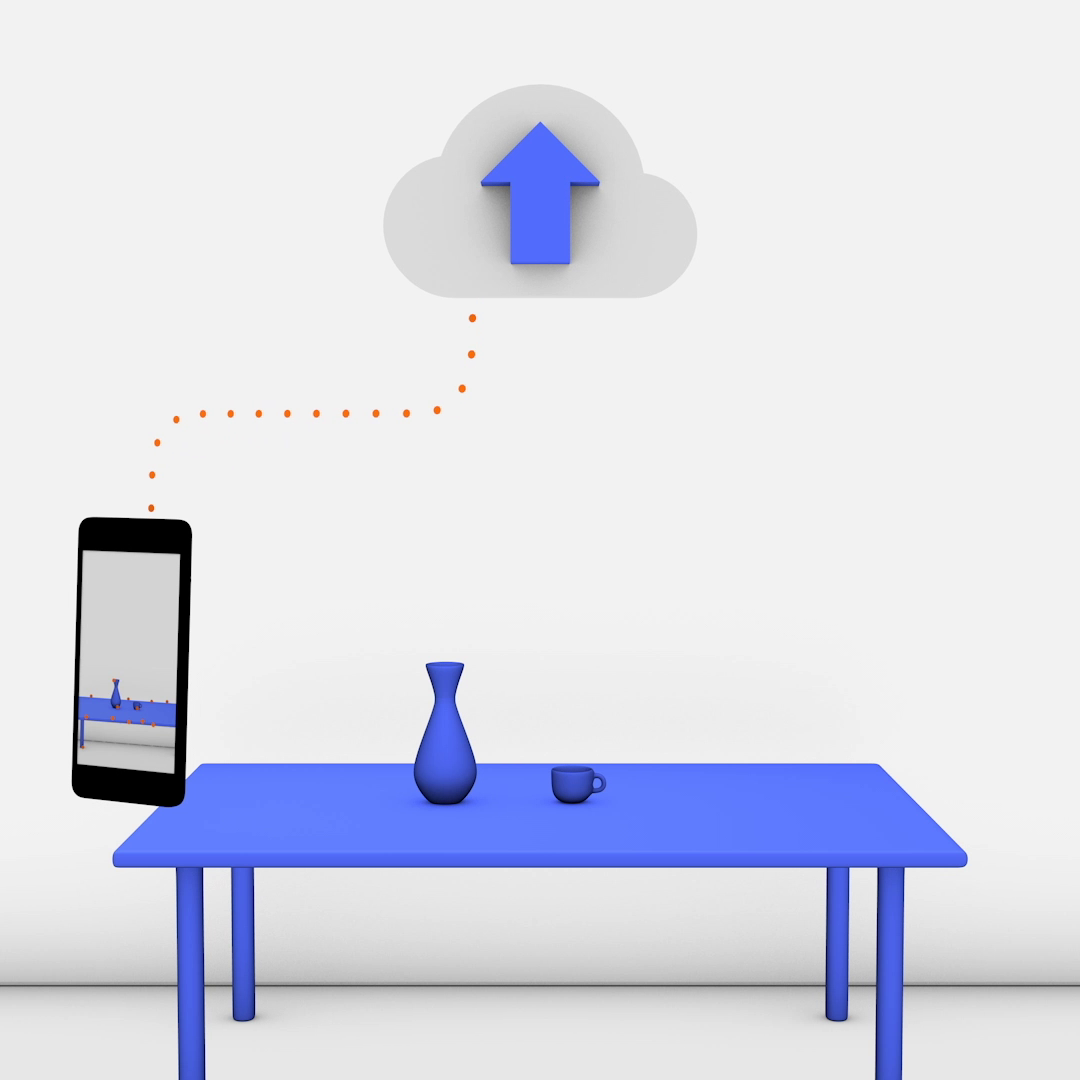
\includegraphics[width=0.45\textwidth]{./resources/images/cloud_anchors/hosting}} \\
		\subfloat[][\emph{Richiesta resolve al cloud anchor.}]
		{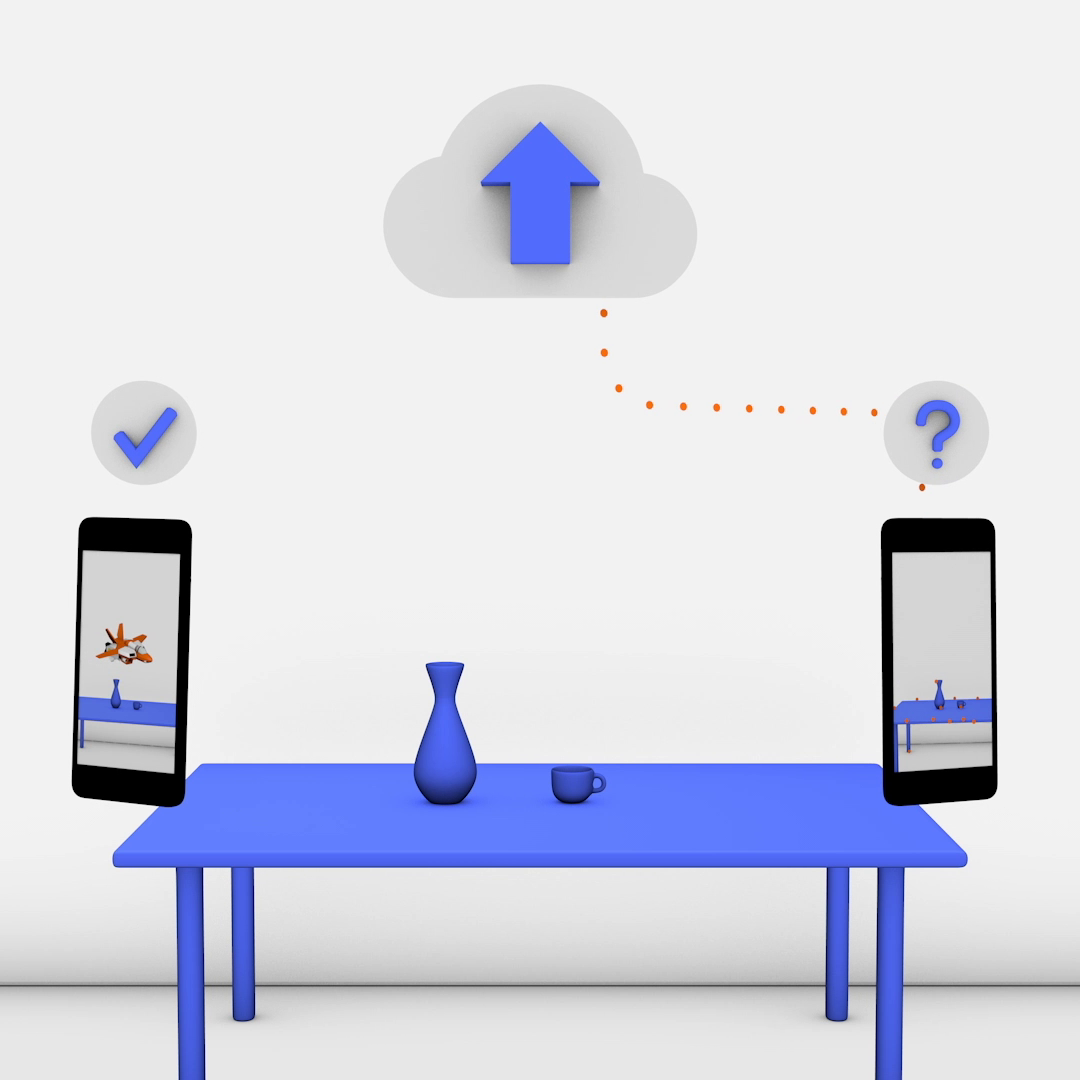
\includegraphics[width=0.45\textwidth]{./resources/images/cloud_anchors/distribution}} \quad
		\subfloat[][\emph{Resolve del cloud anchor.}]
		{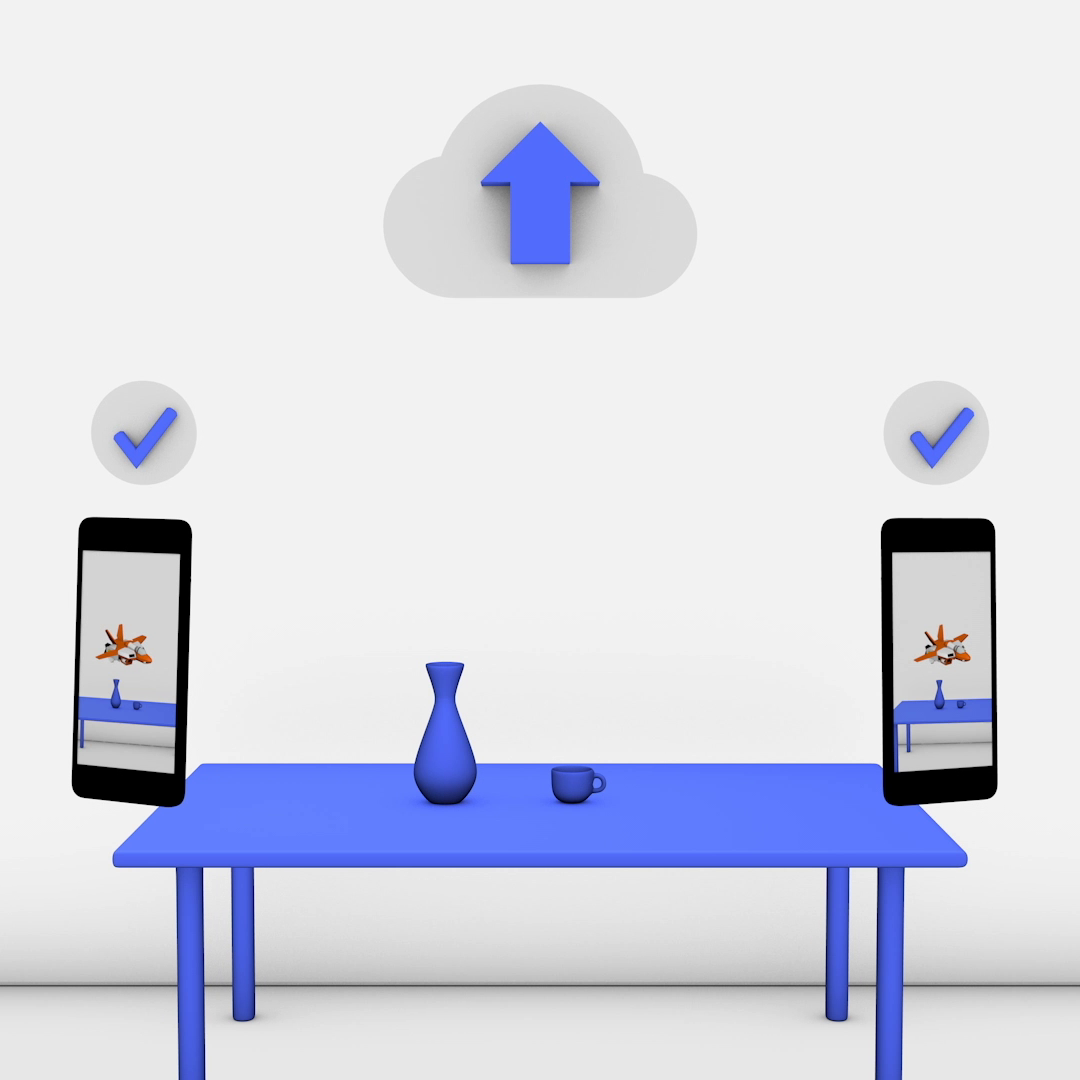
\includegraphics[width=0.45\textwidth]{./resources/images/cloud_anchors/resolving}}
		\caption{Funzionamento ad alto livello di Cloud Anchor API.}
		\label{fig:cloud}
	\end{figure}

	\section{Implementazione e utilizzo}
	Per implementare un'applicazione che utilizzi i Cloud Anchor è prima necessario creare un progetto in \textit{Google Cloud Platform} e abilitare il ARCore Cloud Anchor API per l'hosting, il salvataggio e il resolving degli anchor.
	\\
	\noindent
	La sessione ARCore dell'app deve poter comunicare con il progetto cloud creato, come descritto dal listing~\vref{lst:ca_session} tratto dalla documentazione ufficiale.
	\begin{center}
		\begin{minipage}{0.95\textwidth}
			\begin{lstlisting}[caption={Configurazione della modalità Cloud Anchor.}, label={lst:ca_session}, language=Kotlin]
			val config = Config(session)
			config.cloudAnchorMode = Config.CloudAnchorMode.ENABLED
			session.configure(config)
			\end{lstlisting}
		\end{minipage}
	\end{center}

	Autenticazione...

\end{document}